\documentclass[conference]{IEEEtran}
\IEEEoverridecommandlockouts
% The preceding line is only needed to identify funding in the first footnote. If that is unneeded, please comment it out.
\usepackage{cite}
\usepackage{amsmath,amssymb,amsfonts}
\usepackage{algorithmic}
\usepackage{graphicx}
\usepackage{textcomp}
\usepackage{xcolor}

%KHOA BEGIN
\usepackage{multirow}
\usepackage{array}
%KHOA END

\ifCLASSOPTIONcompsoc
    \usepackage[caption=false, font=normalsize, labelfont=sf, textfont=sf]{subfig}
\else
\usepackage[caption=false, font=footnotesize]{subfig}

\def\BibTeX{{\rm B\kern-.05em{\sc i\kern-.025em b}\kern-.08em
    T\kern-.1667em\lower.7ex\hbox{E}\kern-.125emX}}
\begin{document}

\title{Improving Ultra-Reliable Low-Latency Communication in multiplexing with Enhanced Mobile Broadband\\
%{\footnotesize \textsuperscript{*}Note: Sub-titles are not captured in Xplore and
%should not be used}
%\thanks{Identify applicable funding agency here. If none, delete this.}
}

\author{\IEEEauthorblockN{Trung-Kien Le, Florian Kaltenberger}
\IEEEauthorblockA{\textit{EURECOM} \\
%\textit{name of organization (of Aff.)}\\
Biot, France \\
Emails: first name.last name@eurecom.fr}
\and
\IEEEauthorblockN{Umer Salim}
\IEEEauthorblockA{\textit{TCL Communication} \\
%\textit{name of organization (of Aff.)}\\
Paris, France \\
Emails: umer.salim@tcl.com}
%\and
%\IEEEauthorblockN{3\textsuperscript{rd} Given Name Surname}
%\IEEEauthorblockA{\textit{dept. name of organization (of Aff.)} \\
%\textit{name of organization (of Aff.)}\\
%City, Country \\
%email address}
%\and
%\IEEEauthorblockN{4\textsuperscript{th} Given Name Surname}
%\IEEEauthorblockA{\textit{dept. name of organization (of Aff.)} \\
%\textit{name of organization (of Aff.)}\\
%City, Country \\
%email address}
%\and
%\IEEEauthorblockN{5\textsuperscript{th} Given Name Surname}
%\IEEEauthorblockA{\textit{dept. name of organization (of Aff.)} \\
%\textit{name of organization (of Aff.)}\\
%City, Country \\
%email address}
%\and
%\IEEEauthorblockN{6\textsuperscript{th} Given Name Surname}
%\IEEEauthorblockA{\textit{dept. name of organization (of Aff.)} \\
%\textit{name of organization (of Aff.)}\\
%City, Country \\
%email address}
}

\maketitle

\begin{abstract}
A multiplexing of Ultra-Reliable Low-Latency Communication (URLLC) and Enhanced Mobile Broadband (eMBB) with different requirements in an overlapped time and frequency resources degrades the performance of URLLC and prevents it from attaining the strict requirements of reliability and latency. In this paper, a two-step strategy containing an overlap indication and explicit Hybrid automatic repeat request (HARQ) feedback is proposed to improve URLLC performance in multiplexing with eMBB. Besides explicit HARQ feedback, a scheme with an additional Scheduling Request (SR) to increase diversity of system is also presented.

\end{abstract}

\begin{IEEEkeywords}
5G, URLLC, uplink scheduling scheme, eMBB and URLLC multiplexing, explicit HARQ feedback
\end{IEEEkeywords}

\section{Introduction} \label{I}
One main target of the 5G NewRadio (NR) standard is to support Ultra-Reliable Low-Latency Communication (URLLC) for devices requiring low latency and high link reliability. In \cite{b6}, 3GPP defines targets for the URLLC scenario: ``A general URLLC reliability requirement for one transmission of a packet is 10\textsuperscript{-5} for 32 bytes with a user plane latency of 1 ms''. The next release of 3GPP will have higher requirements of URLLC: ``Higher reliability (up to 10\textsuperscript{-6}), higher availability, short latency in the order of 0.5 to 1 ms, depending on the use cases (factory automation, transport industry and electrical power distribution)''\cite{b8}.

\subsection{Techniques accepted in 3GPP Release 15}\label{IAA}
3GPP Release 15 specified new features in physical layer design to help URLLC achieve the requirements.

Subcarrier spacings (SCS) has a flexible range from 15 kHz to 240 kHz in 5G that results in very short symbol and slot timings\cite{ad2}. In addition, the transmission is scheduled in  mini-slot level in both uplink (UL) and downlink (DL)\cite{ad3}. Due to these features, the network becomes very reactive to users (UEs)' UL and DL traffic demands and the response time to accommodate DL or UL traffic is very small compared to LTE and LTE-Advanced.

Another feature is the standardization of the grant-free (GF)/configured-grant (CG) UL transmissions which allows the UEs to transmit data in the UL direction without having to make an explicit scheduling request (SR) and receiving an UL grant each time before a transmission\cite{ad4}.

\subsection{Problem of multiplexing URLLC and eMBB in GF resources}\label{IBB}
In 5G, a base station (gNB) is able to schedule pre-configured resources (GF/CG resources) for URLLC UEs. But the gNB does not have any prior information which of these GF resources will actually be used by URLLC UEs or which of the UEs in the group configured to the resources will use a specific resource. If the cell is loaded and the gNB schedules some eMBB UEs on the resource overlapping with configured-grant occasion, as shown in Fig.~\ref{fig1}, there is going to be transmission collision of dynamically scheduled eMBB and URLLC GF transmissions. 

\begin{figure}[htbp]
\centerline{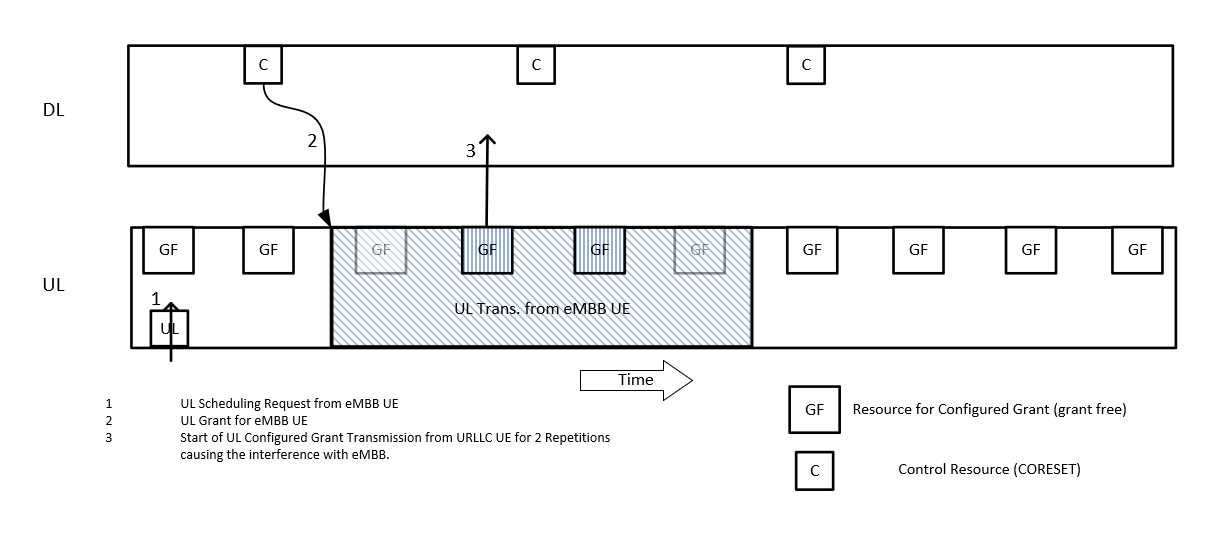
\includegraphics[scale=0.22]{fig1.png}}
\caption{A collision of UL URLLC GF transmission with eMBB transmission in case of FDD.}
\label{fig1}
\end{figure}

When the transmission from eMBB and URLLC UEs in GF resources overlaps, it results in lower decoding probability due to lower resulting SINR for both UEs. This can be a serious problem for URLLC UEs in particular due to their tight latency and reliability targets.

In case the gNB is able to identify the URLLC UE from its DMRS sequence, it may try to quickly reschedule the UE over non-overlapping resources. Thus, it may move the UE from GF to UL grant-based (GB) transmission.

The increased interference due to overlapping transmissions of eMBB and URLLC UEs may lead to situations when the gNB may not even identify the URLLC UE. This situation is particularly catastrophic for URLLC UE. The HARQ structure in UL transmission for NR is timer based, which means that upon transmission of packet, the UE will start the HARQ timer. If it receives an UL grant for the re-transmission of the same transport block (TB) from the gNB, it does the retransmission over the resources scheduled in the UL grant. If it receives no UL grant from the gNB and the HARQ timer expires, it considers that the TB was successfully decoded at the gNB and it discards the data in the buffer. 

The timer based HARQ feedback and UL GB retransmission are standardized because this minimizes the control overhead for sending HARQ feedback. This is reasonable in general but in the cases of dynamic UL multiplexing, giving rise to overlapping transmissions with GF UEs, when the gNB will not be able to identify the UEs transmitting on GF resources, the UEs will discard their packets and consider the successful detection that leads to serious performance degradation for URLLC UEs.

\subsection{Prior art}\label{ICC}
In \cite{b1}, \cite{b2} and \cite{b3}, an UL resource indication is introduced to inform the URLLC UE that the GF resources are already scheduled to the eMBB UE. Upon receiving this indication, the URLLC UE applies a different pre-configured transmission power that is higher than power level used in case of no overlap. Because of the higher transmission power, the gNB has a higher chance to decode correctly URLLC packet from the UE despite the overlapping transmission between the URLLC and eMBB UEs. However, an increase of power causes interference among the neighboring cells. Moreover, this solution is not suitable to the cell-edge UEs because their power is limited.

\cite{b4} and \cite{b5} propose that the gNB assigns URLLC PUSCH with updated transmission parameters such as resource, MCS, transmit power, etc. on grant free resources that are occupied by eMBB PUSCH. This method also poses the problems of interference and power limitation. 

In \cite{b7}, the group common control channel reveals time and frequency resource range allocated to GB eMBB UE, the GF UE can exclude the occupied resource of GB UE based on the this information. Nevertheless, the GF UE has less resources left to transmit than the original configured resources and are obliged to use a higher MCS so it might deteriorate transmission's reliability.

The gNB is proposed to inform the URLLC UE which of the GF resource set has overlapping eMBB transmission such that the URLLC UE can initiate the GF transmission over resources not occupied by the ongoing eMBB transmission. It might result in high latency if all resources in the current occasion are full and the UE must wait until the next transmission occasion\cite{b9}.

In this work, a multiplexing scheme with two-step strategy is presented in Section \ref{II}. The first step comprises of the gNB transmitting an overlap indication whenever it schedules an UL transmission having an overlap with the resources configured to the GF transmissions. The second step of the proposed strategy comprises of making the overlapped transmissions to use explicit HARQ feedback structure. An alternative way of the second step is to make the gNB indicate the UEs to send the SR in parallel to transmit data on the GF resources to improve the reliability. Section \ref{III} shows numerical results and performance evaluation. Finally, Section \ref{IV} is conclusion.

%Firstly, reserved resources and calculations to optimize their sizes are presented in Section \ref{II}. The process allowing the UEs to access to these resources is also discussed. Section \ref{III} shows numerical results obtaining from the equations derived in diverse scenarios. Finally, Section \ref{IV} provides the concluding remarks for this work.

\section{Strategy to multiplex the eMBB and URLLC UEs}\label{II}

\subsection{Overlap indication and explicit HARQ ACK feedback}\label{IIAA}
To overcome the problem of the UL GB eMBB and GF URLLC transmissions as shown in Fig.~\ref{fig1}, a strategy which consists of two steps is implemented. 

In the first step, upon scheduling a GB transmission from the eMBB UE over the GF resources, the gNB sends an indication of resource overlap to the URLLC UEs. As the gNB does not know which of the URLLC UEs configured for GF resources may become active in the current interval, this indication needs to be sent to all UEs who have been configured with the GF resources in the current interval as illustrated in Fig.~\ref{fig2}. Upon receiving this overlap indication, the URLLC UEs are aware of the resources which have been dynamically scheduled for other UEs (the eMBB UEs for example) and in case of transmission, they know that their transmissions will be received with increased interference and trigger a mechanism in the next step to deal with this interference.

\begin{figure}[htbp]
\centerline{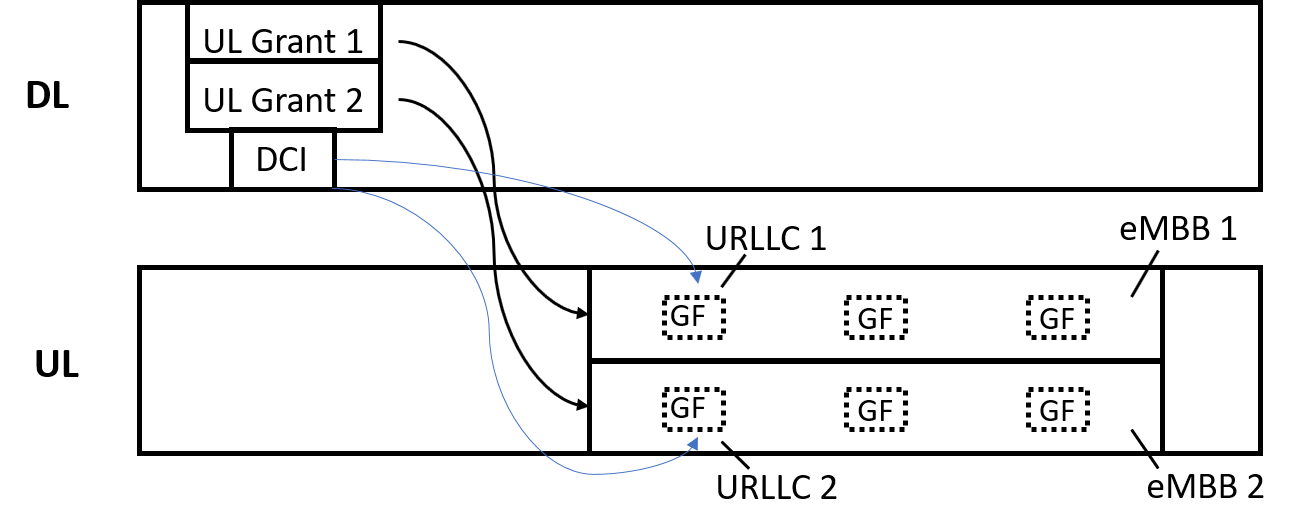
\includegraphics[scale=0.33]{fig2.png}}
\caption{Signalling the URLLC UEs about an overlap with the eMBB UEs in GF regions.}
\label{fig2}
\end{figure}

The second step of the proposed strategy comprises of making the overlapping transmissions use explicit HARQ feedback structure. The resource overlap indication can serve this purpose of making the transmissions explicit HARQ feedback based rather than legacy timer based. Upon receiving this indication, the URLLC UEs, who transmit on the overlapping resources, expect to receive explicit HARQ feedback for their transmissions. 

Thereby, within a configured time period, either the GF UEs receive explicit HARQ ACK indicating the successful detection of their TB or they receive UL grant for re-transmission in case the gNB failed to decode the TB but was able to identify the transmitting UE. For the third case, if the GF UE receives neither an ACK nor an UL grant within a configured time, the UE does not consider that its data is successful, rather it considers that the gNB failed to identify its identity (DMRS detection failure at the gNB) due to high interference in the overlapping transmissions. In this case, the GF UE of interest will do the retransmission of the transport block on the subsequent GF resources.

In addition, the URLLC transmission can be made to stop immediately after receiving an explicit HARQ feedback. Thus, the URLLC UE does not need to carry out all repetitions as configured in parameter repK from higher layer. It helps the URLLC UE save power and resources. Besides, the eMBB UE also avoids suffering from an interference from the URLLC UE’s repetitions and there is more chance that the gNB is still able to decode correctly eMBB data despite the collision with URLLC data at the beginning. 

The timer value, for which the UE should wait to receive ACK or UL grant, can be RRC configured. This value can be selected as a function of reliability and latency targets for the users/applications. For some users/applications with extremely high latency and reliability targets, this timer value can be put to zero which means to do the automatic transmission in case of overlapped transmissions.

In one strategy, it could be decided that all the overlapping GF transmissions use explicit HARQ feedback. In this case, no explicit signalling or flag is needed to indicate the activation of explicit HARQ feedback. Thus, the GF UEs upon knowing that they will transmit on the overlapping resources expect explicit HARQ feedback. There could, though, exist some cases where the gNB knows that it has configured large number of repetitions for GF UEs or it has scheduled the dynamic UL transmission from eMBB UE with a lower power, which will result in a good probability of successful detection or at least UE identification and it decides not to change the HARQ to explicit feedback. To keep the flexible control at the network side, the overlap indication can comprise an indication, a flag, which tells if the feedback becomes explicit or not in the indicated overlapping GF occasions.

\subsection{Overlap indication and additional SR}\label{IIBB}
In a variation of the proposed scheme in Section \ref{IIAA}, the second step of making the transmissions explicit HARQ feedback-based can be altered to use an additional SR. The gNB can indicate the URLLC GF UEs to send a SR in parallel for the TB transmitted over the overlapping GF resources. The SR sent to the gNB will provide a further means - an additional diversity mechanism to the gNB - to react fast to the interfered GF transmission. When the gNB is able to decode the data successfully, it sends some indications to the UE about the successful detection. For the case, when the gNB is unable to identify the UE making the CG transmission, the gNB can react fast to the received SR by sending an UL grant to this UE. Thanks to the UL grant, the UE is likely to retransmit the packet and has a successful transmission in latency budget,

Physical uplink control channel (PUCCH) and physical uplink shared channel (PUSCH) are not allowed to be transmitted simultaneously. In case the UE needs to transmit uplink control information (UCI) while transmitting UL data on PUSCH, it sends the UCI on PUSCH. When the UE is not transmitting PUSCH, it sends the UCI carrying SR, ACK/NAK for DL data, CSI reports etc, on the PUCCH resources using appropriate PUCCH format as a function of UCI content and the PUCCH configurations. The simplest strategy to send SR (which is UCI) when the URLLC UE is transmitting over overlapping GF resources would be to transmit it over PUSCH GF resources along with the transmission of the TB. This can be simple from implementation perspective but from the performance point of view, better performance can be expected if the SR is transmitted using PUCCH configuration on the specified PUCCH resources. As PUCCH resources are dedicated resources on different frequency PRBs and OFDM symbols, this provides additional diversity advantage to the SR transmitted in these resources compared to multiplexing and transmitting it over UL GF resources along with the TB. Therefore, the UE is configured to transmit this SR on PUCCH resources in parallel to the transmission of TB on the overlapping resources.

The overlap indication may have an explicit indication, in the form of a single bit flag, which may require the UEs transmitting over overlapping GF occasions to send SR. In fact, more flexibility and better performance can be achieved by having the flexible control of the explicit HARQ feedback structure and the transmission of SR. The gNB can then choose which strategy to choose in different situations. As an example, if the periodicity of current GF occasions is not very fast, it may make sense to indicate the overlapping GF UEs to send an SR. And in the cases, if the resources configured for SR are not sufficient or not in close proximity compared to the subsequent GF occasions, it may be suitable to prioritize the explicit HARQ feedback and automatic retransmission in case the UEs receive no ACK/NAK/UL-grant indication for the transmitted transport block.

The overlap indication can further be enhanced to modify or update some of the transmission parameters of the GF transmissions which happen to be in the overlap situations such as transmission power level or the number of repetitions. 

\subsection{Configuration and Signalling for the Overlap Indication}\label{IICC}
One very important feature of the proposed scheme is that the overlap indication is sent to the UEs who have been pre-configured for the GF resources. As GF resources may be shared by multiple UEs, and the gNB has no idea a priori which of these UEs may transmit their data over GF resources, this overlap indication is sent in a group-common manner. Thus, the proposal is to send the overlap indication in a group-common downlink control information (DCI).

For overlap indication sent in group-common DCI, the DCI format 2\_1 in \cite{ad6}, which is used for DL pre-emption indication, can be used for UL overlap indication. The size of DCI format 2\_1 is configurable by higher layers up to 126 bits and each indication has 14 bits. 

The UL overlap indication sent to the URLLC UEs comprises of the indication of UL GF resources typically scheduled for the eMBB UEs. The eMBB UEs would be normally scheduled for the slot duration or most part of the valid DL symbols so it would be judicious to have more bits of UL reference resource field defining the frequency granularity. To keep a format close to the DL pre-emption indication and adapted to indicate the UL overlap resource, there are two possibilities of UL overlap indication. In the first design, all 14 bits are used to indicate the frequency PRB region for the whole slot. Thus, each bit in the 14-bit long bitmap indicates 1/14 of the frequency PRBs of the carrier as shown in left part of Fig.~\ref{fig3}. The second option is to split the time-frequency grid of the slot in 7 frequency zones each spanning one half slot. Thus, each bit may indicate an overlap over 1/7 of the frequency PRBs for a half slot time duration as illustrated in right part of Fig.~\ref{fig3}. 

\begin{figure}[htbp]
\centerline{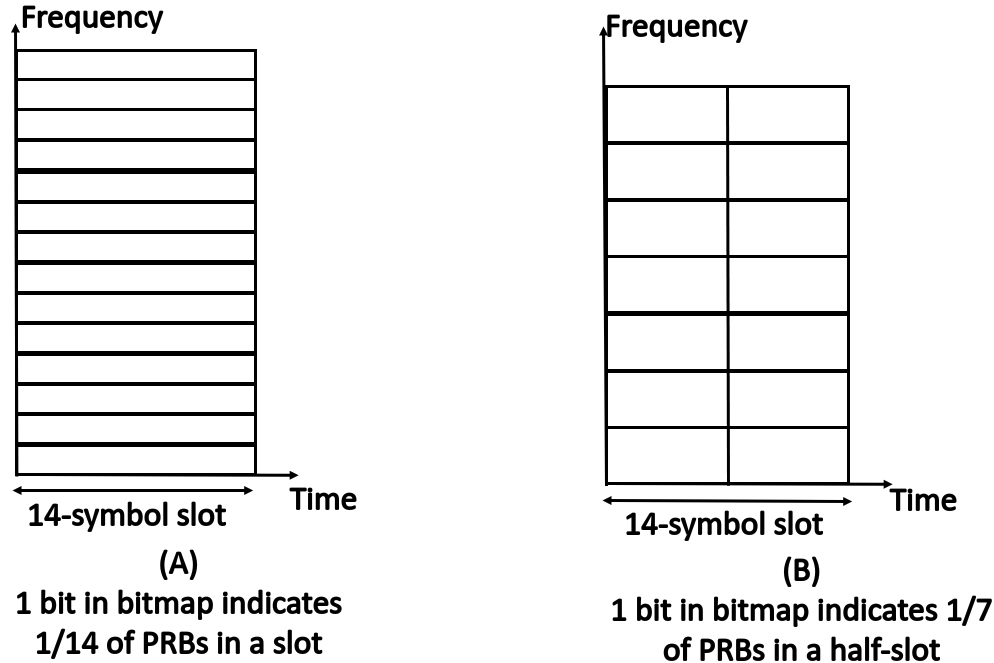
\includegraphics[scale=0.2]{fig3.png}}
\caption{Resource Indication in Uplink Overlap Indication.}
\label{fig3}
\end{figure}

The UEs configured with GF resources can be configured to listen and decode the overlap indication as part of GF configuration. The activation or de-activation of this operation can be done in different ways for Type 1 and Type 2 GF as specified in \cite{ad4}. For RRC configured Type 1, the activation and de-activation can be done by RRC signalling. For configured grant Type 2, where some parameters of GF can be updated by DCI, the activation or de-activation of overlap indication can be made through DCI signalling which is used to update other GF parameters.

The overlap indication can be sent at the same time when the gNB sends the dynamic UL grant scheduling a UE over the GF resources as shown in the left part of Fig.~\ref{fig4}.

When the gNB sends an UL grant scheduling an eMBB UE, the scheduled resources are not necessarily in the same slot where UL grant is sent. Rather typically the UL grant will be for the resources located in one of the subsequent slots. If base station transmits the overlap indication along with the UL grant, it needs to indicate the slot where this overlap will occur. To avoid this additional signalling and to keep the treatment of UL grant simple, the overlap indication can be transmitted in the slot where overlap occurs as shown in the right part of Fig.~\ref{fig4}. However, it may not be preferable to send and receive at the same time, so transmitting the overlap indication in the DL direction in the same slot as of the overlapping CG occasions may not be very interesting. In some other cases like TDD operation mode, it may be completely impossible. Thus, based on the system design, one of these two transmission scheme is determined.

\begin{figure}[htbp]
\centerline{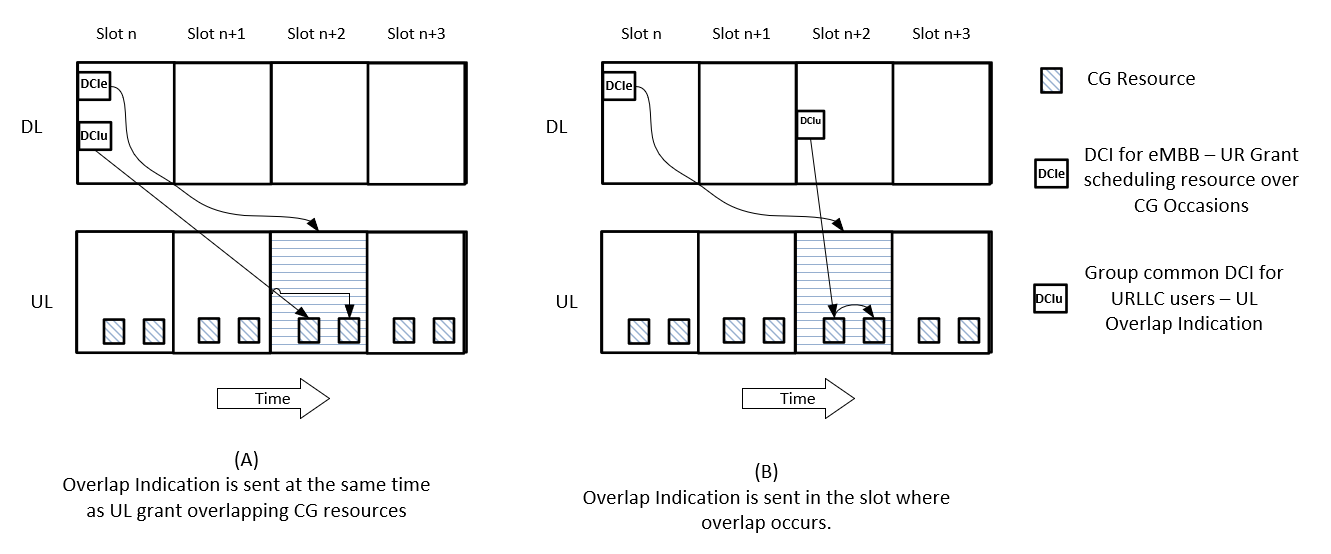
\includegraphics[scale=0.2]{fig4.png}}
\caption{Timing to send the UL Overlap Indication.}
\label{fig4}
\end{figure}

\subsection{Design of Explicit HARQ Feedback}\label{IIDD}
In the proposed strategy, the base station shifts the GF transmissions in the overlap region from timer-based approach to explicit-HARQ-feedback approach. Thus, a design for the explicit HARQ feedback in general may be needed. The proposal is to use DCI as an explicit HARQ feedback. This DCI can be sent with UE specific CS-RNTI which is used with configured grant-based transmissions. If the gNB is able to successfully decode the data despite the overlap, it can send an UL grant to this UE with the same HARQ process number (HARQ ID) as of the successfully received transport block, and the UE upon receiving this UL grant would know that this is in fact not a re-transmission request but an explicit ACK for the previously transmitted transport block. To avoid any confusion, new-data-indicator (NDI) field can be set to zero. Further, some of the fields in the DCI which are actually not needed, such as the time and frequency resource assignment fields, may be sent with fixed known values which can be pre-decided to be used in the ACK indication.

If the gNB fails to decode the transport block but is able to identify the UE through DMRS identification, it sends an UL grant for re-transmission with meaningful resource assignments allowing the UE a quick re-transmission possibility and higher probability to fulfill its latency-reliability targets.

If the gNB even fails to identify the UE due to high interference, it would not be able to schedule the UE for a re-transmission. This is the scenario where explicit HARQ feedback becomes the most promising. If the UE does not receive any re-transmission request because the gNB even failed to identify the UE, upon HARQ timer expiry, it will discard the packet and consider that it was successfully decoded at the gNB so the classic timer-based HARQ structure fails completely. Thus, in the proposed approach, if the UE receives neither an ACK or re-transmission grant, it considers that the gNB failed to identify the UE and re-transmits the same transport block in the subsequent GF resource.

\section{Numerical results and performance evaluation}\label{III}

\begin{table}[htbp]
\caption{Simulation parameters}
\begin{center}
\begin{tabular}{|p{8em}|p{8em}|}
 \hline
 \textbf{Parameters} & \textbf{Values}\\
 \hline
 Waveform & CP-OFDM\\
 \hline
 Subcarrier spacing & 60kHz\\
 \hline
 Channel model & Rician\\
 \hline
 K factor & 1\\
 \hline
 Number of allocated PRB & 8\\
 \hline
 DMRS detection mechanism & Time-domain correlation\\
 

%  increase row height, number of & = number of collumn
% &&&&&\\[-1em]
 
 \hline
\end{tabular}
\label{tab1}
\end{center}
\end{table}

\begin{figure}[htbp]
\centerline{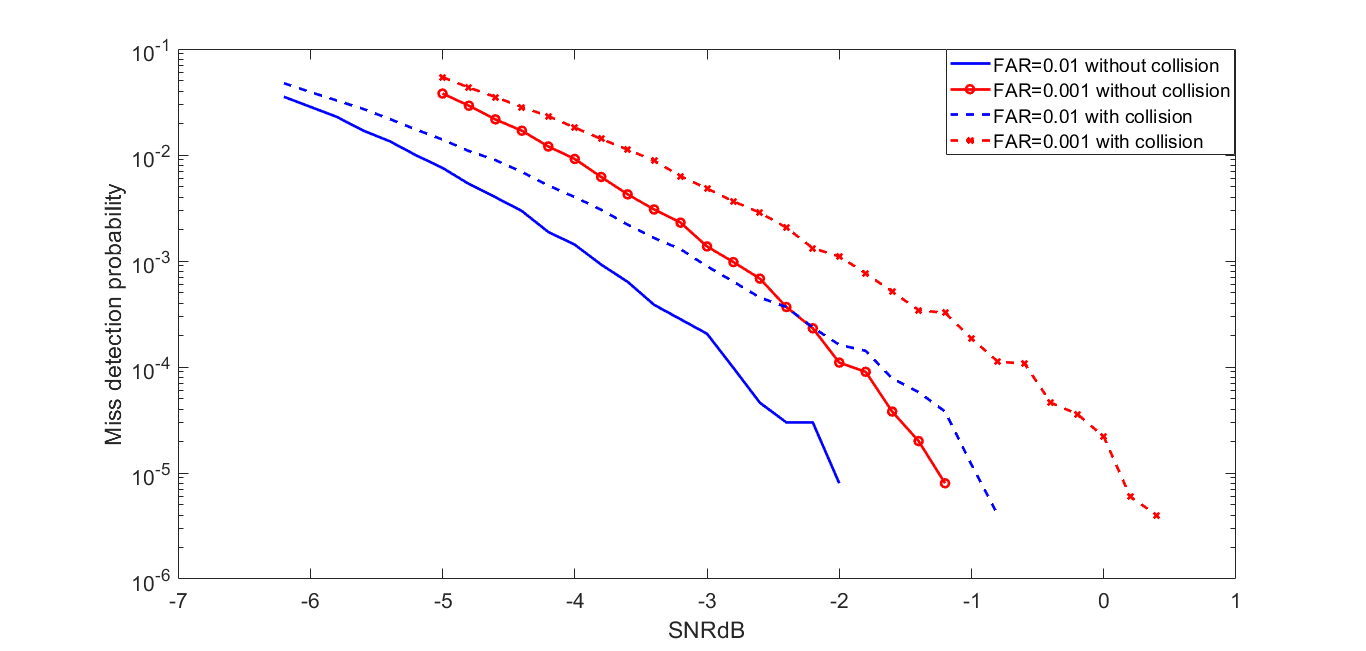
\includegraphics[scale=0.4]{fig5.png}}
\caption{DMRS detection performance.}
\label{fig5}
\end{figure}

Simulation parameters are shown in Table~\ref{tab1}. Fig.~\ref{fig5} illustrates the performance of DMRS detection in two cases: no collision and having a collision with data/DMRS of another UE. For each DMRS detection, the correlation result is compared with a threshold to determine whether DMRS exists or not. This threshold is chosen according to a target false alarm rate (FAR) indicating the cases that the gNB determines the existence of DMRS while in reality there is no DMRS transmitted. A higher threshold is required for a lower FAR but also results in more missed detection.

Due to a collision between DMRS of the UE of interest and data/DMRS of another UE, the performance of DMRS detection degrades significantly as can be seen in Fig.~\ref{fig5} and cannot achieve the miss detection probability 10\textsuperscript{-5} at the same SNR level of the case without collision. At FAR of 0.001 and SNR of -1.4dB, the miss detection probability increases from 10\textsuperscript{-5} to 3.4$\times$10\textsuperscript{-4}. As UE detection to decode and reschedule data if necessary depends on DMRS detection, a degradation of DMRS detection makes the system not be able to support stringent reliability URLLC requirement.

The usage of an explicit HARQ feedback as explained in Section \ref{IIAA} solves the problem of DMRS miss-detection and helps the system achieve the same reliability as the case of no collision between URLLC and eMBB UEs because of the ability of carrying out the retransmissions even if DMRS is not detected by the gNB. Table~\ref{tab2} shows a remarkable enhancement of UL transmission with explicit HARQ feedback in case of URLLC and eMBB multiplexing. Besides that, Table~\ref{tab2} also shows an improvement of UE detection and UL transmission reliability when an additional UL grant is transmitted in parallel with data in GF resources.
 

\begin{table}[htbp]
\caption{Performance comparison between different scenarios and schemes}
\begin{center}
\begin{tabular}{|p{8em}|p{8em}|p{8em}|}
 \hline
 \textbf{Case} & \textbf{UE miss detection probability}& \textbf{UL transmission's BLER}\\
 \hline
 No collision & 10\textsuperscript{-5}&10\textsuperscript{-5}\\
 \hline
 Collision without explicit feedback & 3.4$\times$10\textsuperscript{-4}&3.5$\times$10\textsuperscript{-4}\\
 \hline
 Collision with explicit feedback& 3.4$\times$10\textsuperscript{-4}&10\textsuperscript{-5}\\
\hline
 Collision with additional SR& 1.32$\times$10\textsuperscript{-4}&1.43$\times$10\textsuperscript{-4}\\

%BLER_trans=P_DMRS+(1-P_DMRS)*P_data
%  increase row height, number of & = number of collumn
% &&&&&\\[-1em]
 
 \hline
\end{tabular}
\label{tab2}
\end{center}
\end{table}

The presence of retransmission in explicit feedback or additional SR strategy leads to latency and resource consumption but guarantees target reliability in case of DMRS miss-detection, while the conventional scheme stops the transmission straightaway and causes packet loss so latency and resource consumption have no meaning when a packet is already failed to be decoded correctly. Moreover, with SCS 60kHz and the decoding time of one transmission being 0.1ms for a packet spreading in 4 OFDM symbols, a transmission consumes approximately 1 slot equal to 0.25ms. Thereby, even with one retransmission, the system consumes 0.5ms in total and still satisfies the latency requirement of 1ms.

\section{Conclusion}\label{IV}

This paper presents a strategy to multiplex the GB eMBB and GF URLLC transmission while guaranteeing the strict time and latency requirements of URLLC. An overlap indication is used and combined with an explicit HARQ feedback or an additional SR to counter the harmful effect of interference in multiplexing.

\begin{thebibliography}{00}

\bibitem{b1}  ZTE, ``On UL inter UE Tx prioritization/multiplexing'', 3GPP R1-1812389, RAN1\#95, Spokane, USA, November 12--16, 2018.
\bibitem{b2} Huawei, HiSilicon, ``UL inter-UE transmission prioritization and multiplexing'', 3GPP R1-1810158, RAN1\#94bis, Spokane, Chengdu, China, 8--12 October, 2018.
\bibitem{b3} ZTE, ``UL inter-UE multiplexing between eMBB and URLLC'', 3GPP R1-1900074, RAN1 AH 1901, Taipei,  21--25 January, 2019.
\bibitem{b4} Sony, ``On Enhancement of UL grant-free transmissions'', 3GPP R1-1808345, RAN1\#94, Gothenburg, Sweden, August 20--24, 2018.
\bibitem{b5}  Sony, ``Inter-UE uplink multiplexing of URLLC \& eMBB traffics'', 3GPP R1-1812745, RAN1\#95, Spokane, USA, November 12--16, 2018.
\bibitem{b7}  Institute for Information Industry (III), ``UL Inter UE Tx prioritization/multiplexing'', 3GPP R1-1813481, RAN1\#95, Spokane, USA, November 12--16, 2018.
\bibitem{b9}  NEC, ``UL inter-UE multiplexing of eMBB and URLLC'', 3GPP R1-1812419, RAN1\#95, Spokane, USA, November 12--16, 2018.

\bibitem{b6} 3GPP TR 38.913 v15.0.0, ``Study on scenarios and requirements for next generation access technologies.''
\bibitem{b8} Huawei, HiSilicon, Nokia, Nokia Shanghai Bell, ``New SID on Physical Layer Enhancements for NR URLLC''. 3GPP RP-182089, TSG-RAN\#81, Gold Coast, Australia, Sept 10--13, 2018.
\bibitem{ad2} 3GPP TS 38.211 v15.3.0, ``Physical channels and modulation.''
\bibitem{ad3} 3GPP TR 38.802 v14.2.0, ``Study on new radio access technology physical layer aspects.''
\bibitem{ad4} 3GPP TS 38.214 v15.3.0, ``Physical layer procedures for data.''
\bibitem{ad6} 3GPP TS 38.212 v15.3.0, ``Multiplexing and channel coding.''

\end{thebibliography}
\vspace{12pt}


\end{document}
